\chapter{Fundamente de fiabilitate, redundanţă şi mentenabilitate}
\thispagestyle{pagestyle}
Necesitatea de a menține funcționarea continuă și optimă a sistemelor embedded a condus la dezvoltarea unor principii esențiale pentru implementarea acestor sisteme. Pentru ca un sistem să răspundă cerințelor pentru care a fost creat, nu este suficient să își îndeplinească funcțiile. Acesta trebuie să fie fiabil, să mențină un echilibru adecvat între cost și eficiență și să fie ușor de întreținut.

\section{Fiabilitate}
Fiabilitatea (notată cu R(t)) se referă la abilitatea unui sistem sau a unei componente de a funcționa fără defecțiuni pe o durată de timp specificată (intervalul de timp [$t_0$,t])
 și în condiții de utilizare definite. Aceasta este o trăsătură crucială, deoarece are un impact direct asupra performanței și disponibilității sistemului. Un sistem fiabil reduce la minimum perioadele de nefuncționare și costurile de întreținere, consolidând totodată încrederea utilizatorilor în capacitatea sa de a opera conform specificațiilor stabilite\cite{fiabilitate_curs}, \cite{fault_tolerant}.

 Pentru a asigura un nivel înalt de fiabilitate, este esențial să se efectueze o proiectare minuțioasă, să se utilizeze componente de înaltă calitate și să se desfășoare teste riguroase. Suplimentar, monitorizarea constantă și întreținerea preventivă sunt vitale pentru a menține fiabilitatea pe termen lung. În domeniul sistemelor embedded, fiabilitatea capătă o importanță majoră, deoarece aceste sisteme sunt frecvent implementate în aplicații critice, unde defecțiunile pot avea impacturi semnificative.

 Pentru dispozitivele complexe, respectarea principiului fiabilității implică poziționarea componentelor într-un sistem în două perspective:

\begin{itemize}
\item Din punct de vedere fiabilistic: se subliniază că fiabilitatea unei componente din cadrul sistemului poate influența fiabilitatea altor componente.
\item Din punct de vedere structural: se analizează fiabilitatea sistemului în funcție de aranjarea componentelor.
\end{itemize}


Există patru modalități principale de configurare a componentelor \cite{fault_tolerant}:

\begin{itemize}
\item Serie: Defectarea unei singure componente cauzează defectarea întregului sistem.
\item Paralel: Sistemul continuă să funcționeze până când ultima componentă se defectează; defectarea întregului sistem are loc doar dacă toate componentele se defectează.
\item Serie-paralel: Întregul sistem se defectează numai dacă toate componentele dispuse în paralel se defectează.
\item Paralel-serie: Sistemul se defectează complet dacă toate componentele dispuse în serie se defectează.
\end{itemize}

Luând în considerare aspectele prezentate mai sus, am decis ca în sistemul proiectat de mine să folosesc o dispunere în paralel a componentelor pentru a asigura o fiabilitate cât mai ridicată. O defecțiune la o anumită componentă nu va duce la distrugerea întregului sistem și îi va permite o funcționare parțială, dar totuși relevantă.


\section{Mentenabilitate}


Mentenabilitatea, proprietatea unui sistem de a fi întreținut și reparat cu ușurință, este crucială pentru a asigura funcționarea continuă și eficientă pe termen lung. Aceasta poate fi definită atât calitativ, cât și cantitativ. Din perspectivă calitativă, mentenabilitatea se referă la capacitatea unui sistem de a funcționa fără defecțiuni într-o anumită perioadă de timp. Din punct de vedere cantitativ, aceasta reprezintă capacitatea sistemului de a îndeplini funcțiile pentru care a fost implementat \cite{fault_tolerant}.

Mentenabilitatea include atât întreținerea preventivă, care are ca scop evitarea defecțiunilor prin inspecții și ajustări regulate, cât și întreținerea corectivă, concentrată pe repararea sau înlocuirea componentelor defecte după apariția unei probleme. Este esențială în proiectarea sistemelor, influențând direct costurile de operare și timpul de nefuncționare.

Un sistem cu o mentenabilitate ridicată permite tehnicienilor să identifice rapid problemele, să acceseze cu ușurință componentele necesare pentru reparații și să finalizeze lucrările necesare într-un interval de timp scurt. Proprietatea de mentenabilitate devine foarte importantă în perioada de maturitate a produsului, după ce acesta a fost introdus pe piață și pus în funcțiune, deoarece este principalul factor care trebuie luat în calcul pentru a menține performanțele sistemului și pentru a minimiza costurile și timpul de nefuncționare.

Astfel, în sistemul creat de mine componentele pot fi înlocuite individual, fără a fi nevoie ca întreg sistemul să fie dezasamblat. Atât timp cât dispunem de componente noi pentru înlocuirea celor defectate, timpul de nefuncționare ar trebui să fie de ordinul minutelor.

\section{Redundanţă}
Redundanța implică adăugarea de componente suplimentare sau sisteme alternative într-un design pentru a îmbunătăți fiabilitatea și disponibilitatea acestuia. Atunci când apare o defecțiune, aceste elemente redundante preiau funcțiile componentelor defecte, garantând continuitatea operării sistemului \cite{fault_tolerant}.

Putem avea 4 modalități de implementare a redundanței:

\begin{itemize}
\item Hardware
\item Software
\item Informațional
\item Temporal
\end{itemize}

Redundanța hardware constă în folosirea unor echipamente suplimentare, cum ar fi surse de alimentare, procesoare sau unități de stocare duplicate. Redundanța software presupune implementarea unor algoritmi sau programe alternative capabile să preia controlul în cazul unei erori a software-ului principal. Redundanța informațională implică replicarea și distribuirea datelor pe multiple suporturi sau locații pentru a preveni pierderea acestora. Redundanța temporală se referă la executarea unor operații sau procese critice în momente diferite, asigurând astfel, că în cazul unui eșec inițial, există posibilitatea reîncercării fără a compromite funcționarea generală a sistemului.

În sistemul creat de mine am implementat atât redundanță hardware, cât și informațională. Redundanța hardware provine din faptul că datele adunate de senzori sunt transmise atât prin Bluetooth către aplicația mobilă creată de mine, prin WiFi către Cloud-ul Blynk unde se pot urmări folosind aplicația web sau mobile oferită de aceștia și nu în ultimul rând pe LCD-ul atașat sistemului. Astfel, dacă una sau două dintre căile de vizualizare a datelor se defectează încă este posibil ca sistemul să fie supravegheat. Redundanța informațională este oferită cu ajutorul Cloud-ului Blynk, unde informațiile înregistrate până la momentul defectării sau al statusului de offline, sunt înregistrate și pot fi exportate.

\section{Fault Tree Analysis}
Fault Tree Analysis (FTA) este o metodă deductivă utilizată pentru a identifica și evalua cauzele potențiale ale defecțiunilor în sistemele complexe. Această tehnică ajută la determinarea modului în care diverse defecțiuni ale componentelor pot duce la o defecțiune generală a sistemului. Aceste defecțiuni neplăcute pot fi cauzate de probleme software, hardware sau de erori umane \cite{fiabilitate_curs}.

Metoda deductivă începe cu o concluzie generală și se focalizează pe identificarea cauzelor specifice până la cel mai detaliat element care poate contribui la acea concluzie. Prin acest proces, se construiește un arbore al defecțiunilor provenite din cauze multiple sau simple.

Scopul principal al analizei acestui arbore este de a ajuta la identificarea cauzelor potențiale de defectare a sistemului înainte ca acestea să se producă efectiv.

Pentru a detecta cauzele defecțiunii este folosit arborele din Figura \ref{fig:fta}. Modul de parcurgere al acestuia este de sus în jos și este interpretat pe nivele. Evenimentul principal este \texttt{System failure} (Defectarea sistemului) și folosind poarta \texttt{OR}, acestă defecțiune poate apărea din două motive: \texttt{sensor failure} (defecțiunea senzorilor) sau \texttt{Control boards failure} (defecțiunea plăcilor de control). La rândul lor, aceste două defecțiuni pot apărea din varii motive. Defecțiunea senzorilor poate apărea dintr-o lipsă de alimentare sau dintr-o interpretare incorectă a datelor. Defecțiunea plăcilor de control poate fi determinată de o eroare software în codul rulat sau de o eroare de hardware care poate apărea la rândul ei din alte două motive: lipsa alimentării sau o eroare a microcontroler-ului.

\begin{figure}[H]
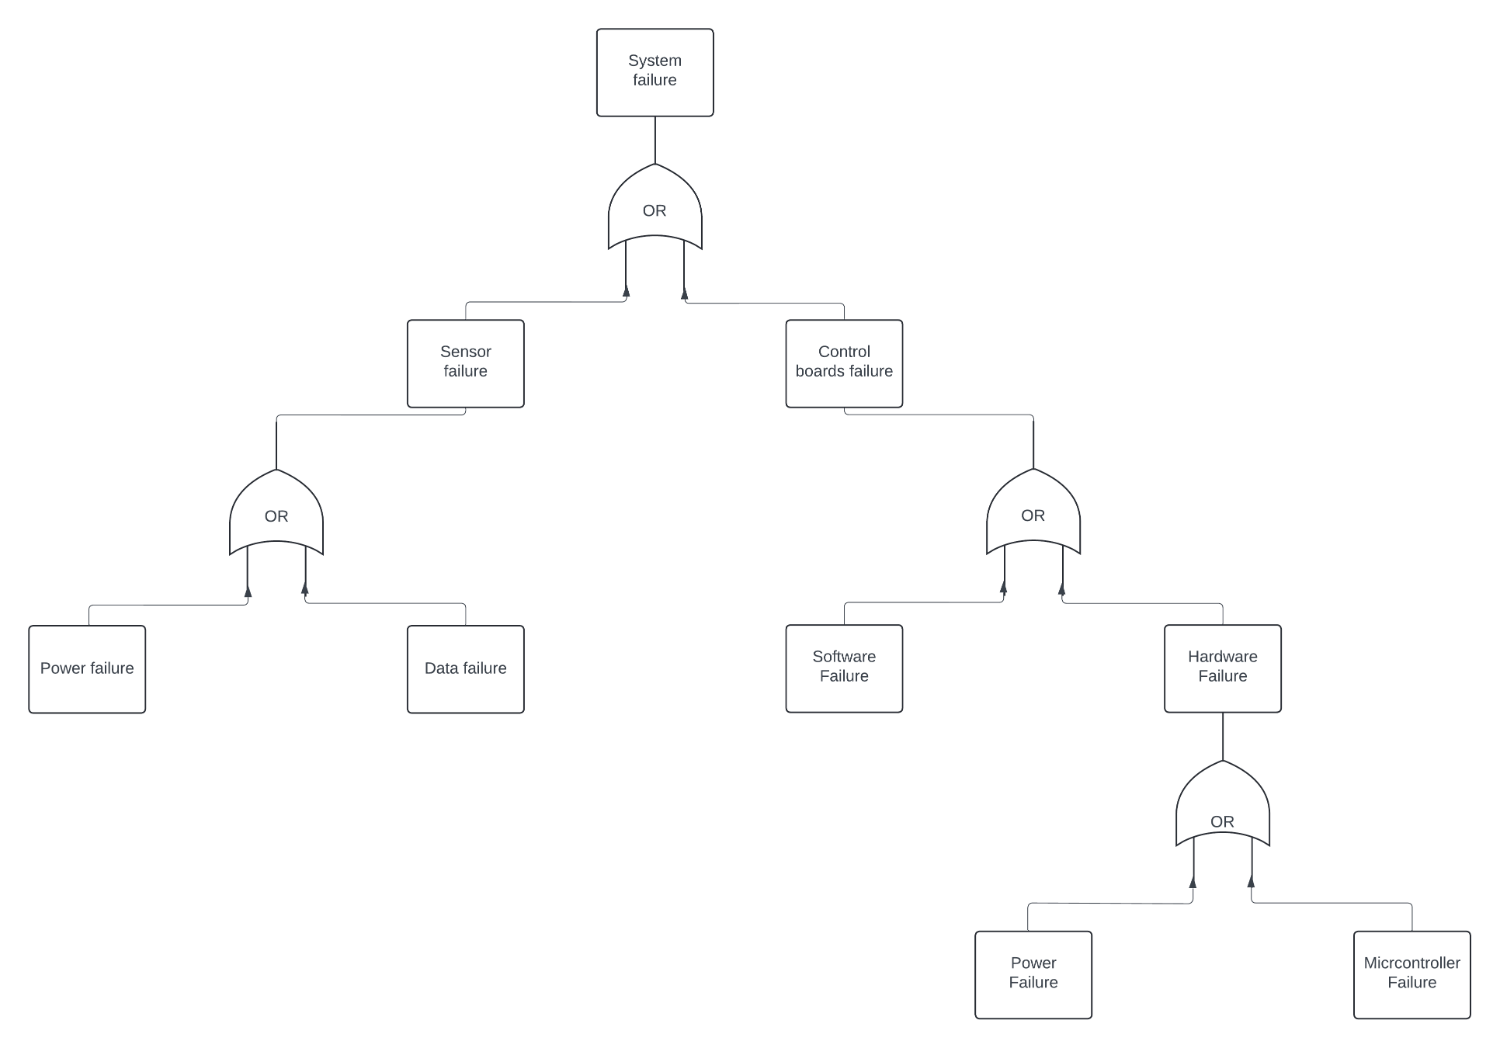
\includegraphics[width=1\linewidth]{images/fta.png}
\caption{Fault Tree Analysis pentru sistemul implementat}
\label{fig:fta}
\end{figure}

